% Created 2021-10-16 sáb 21:33
% Intended LaTeX compiler: pdflatex
\documentclass[11pt]{article}
\usepackage[utf8]{inputenc}
\usepackage[T1]{fontenc}
\usepackage{graphicx}
\usepackage{grffile}
\usepackage{longtable}
\usepackage{wrapfig}
\usepackage{rotating}
\usepackage[normalem]{ulem}
\usepackage{amsmath}
\usepackage{textcomp}
\usepackage{amssymb}
\usepackage{capt-of}
\usepackage{hyperref}
\usepackage{fullpage}
\author{martín rossi}
\date{}
\title{trábajo práctico ipv6}
\hypersetup{
 pdfauthor={martín rossi},
 pdftitle={trábajo práctico ipv6},
 pdfkeywords={},
 pdfsubject={},
 pdfcreator={Emacs 27.2 (Org mode 9.4.4)}, 
 pdflang={English}}
\begin{document}

\maketitle
\begin{enumerate}
\item c.
\begin{center}
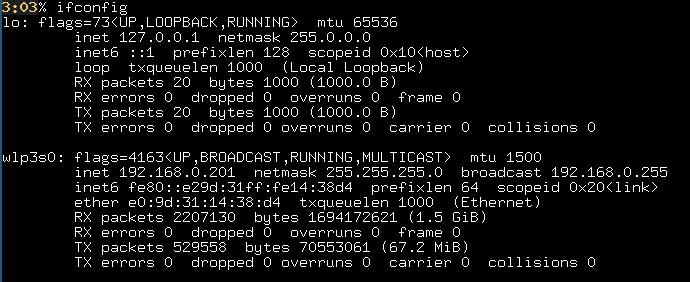
\includegraphics[width=.9\linewidth]{./1c.png}
\end{center}
Primero se ve la interfaz loopback (lo) con direcciones 127.0.0.1 y ::1 para IPv4 e IPv6.

Después se ve otra interfaz wlp3s0, que tiene dirección IPv6 fe80::e29d:31ff:fe14:38d4 con el prefijo fe80 que indica una dirección link local, o sea que es válida sólo para el enlace local. Su dirección MAC es e0:9d:31:14:38:d4.

d.
\begin{center}
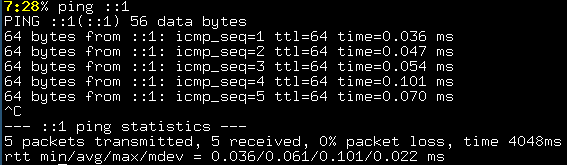
\includegraphics[width=.9\linewidth]{./1d.png}
\end{center}

e.
Acá hice un ping con un celular conectado al mismo router que la computadora pero con IPv4.

\begin{center}
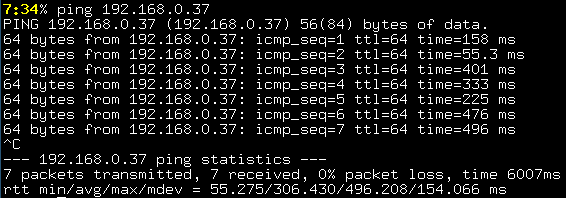
\includegraphics[width=.9\linewidth]{./1ea.png}
\end{center}
\begin{center}
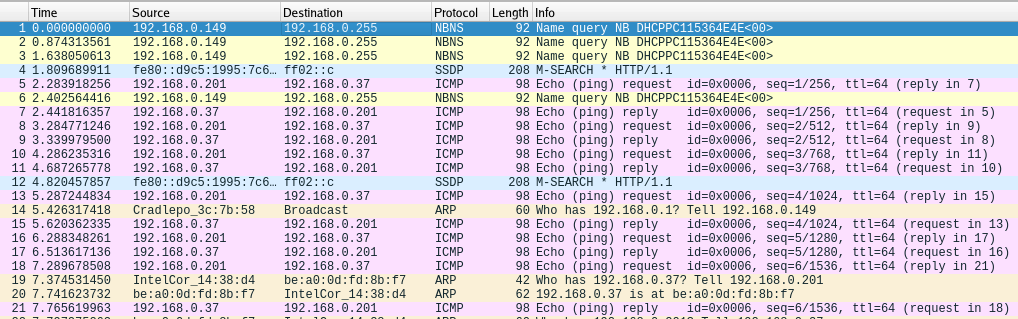
\includegraphics[width=.9\linewidth]{./1eb.png}
\end{center}

Se pueden ver los paquetes ICMP en rojo de los ping request y reply entre 192.168.0.37 y 192.168.0.201. La información adicional que se muestra es el id del mensaje ping, el número de secuencia y el time to live (ttl).

f.
\begin{center}
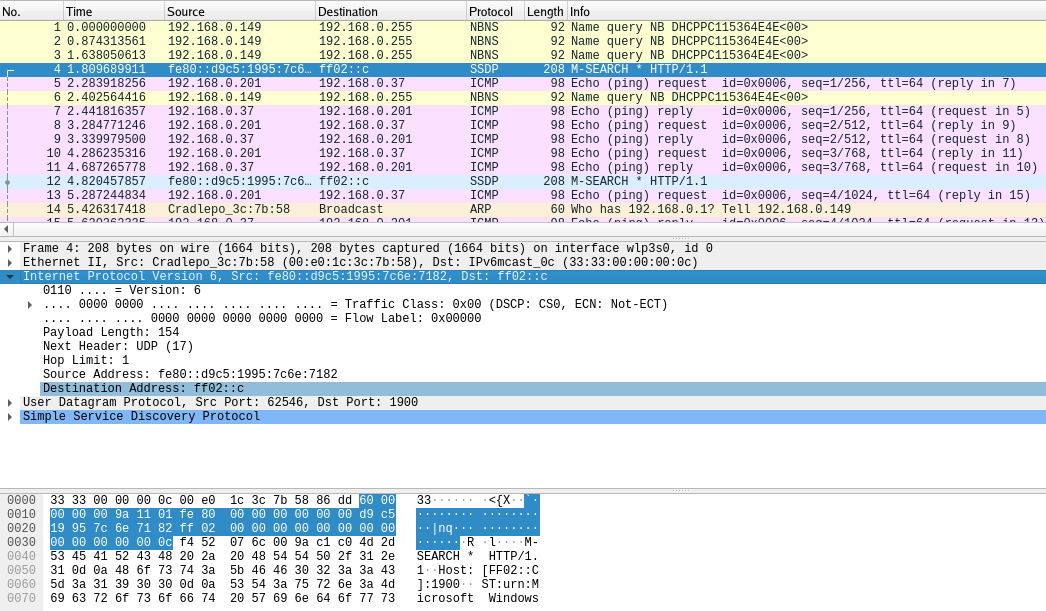
\includegraphics[width=.9\linewidth]{./1f.png}
\end{center}
Se puede ver que la cabecera del paquete tiene los campos
\begin{itemize}
\item versión: 0110 (6)
\item trafic class: 0x00
\item flow label: 0x00000
\item payload length: 154
\item next header: 17 (UDP)
\item hop limit: 1
\item source address
\item destination address
\end{itemize}

g.
\begin{center}
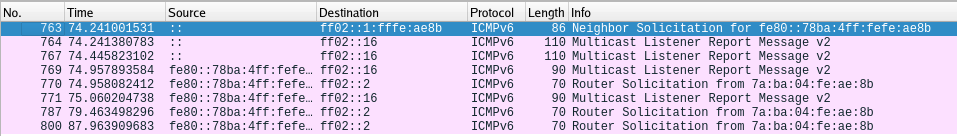
\includegraphics[width=.9\linewidth]{./1g.png}
\end{center}

Cuando se conecta un nodo nuevo se intercambian mensajes de descubrimiento de vecinos. Los mensajes son:
\begin{itemize}
\item \textbf{Neighbor Solicitation:} tipo 135. Se usa para determinar direcciones MAC de los vecinos.
\end{itemize}
\begin{center}
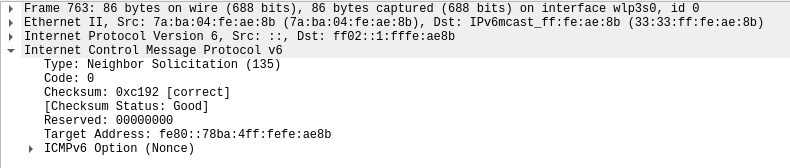
\includegraphics[width=.9\linewidth]{./1ga.png}
\end{center}
\begin{itemize}
\item \textbf{Multicast Listener Report Message:} tipo 143. Es para descubrir nodos que deseen recibir paquetes multicast.
\end{itemize}
\begin{center}
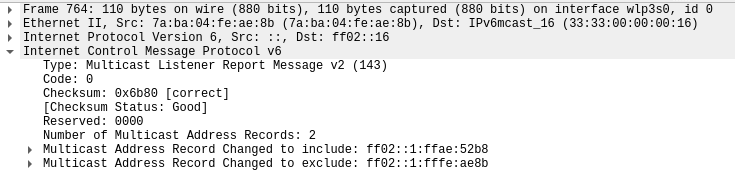
\includegraphics[width=.9\linewidth]{./1gb.png}
\end{center}
\begin{itemize}
\item \textbf{Router Solicitation:} tipo 133. Cuando un nodo nuevo se conecta pide al router que se anuncie para informar a los nodos.
\end{itemize}
\begin{center}
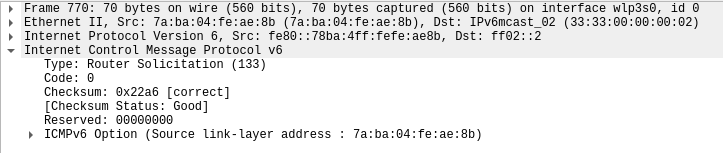
\includegraphics[width=.9\linewidth]{./1gc.png}
\end{center}

\item Tarea 2.

b.

Las 4 interfaces tienen IPv6 habilitado
\begin{center}
\begin{tabular}{llll}
\textbf{Dispositivo} &  & \textbf{Dirección IP local} & \textbf{Dirección IP global}\\
\hline
\textbf{Router0} & \textbf{Fa0/0} & FE80::202:4AFF:FE35:6301 & 2001:DB8:1:0:202:4AFF:FE35:6301\\
 & \textbf{Fa0/1} & FE80::202:4AFF:FE35:6302 & 2001:DB8:2:0:202:4AFF:FE35:6302\\
\hline
\textbf{Router1} & \textbf{Fa0/0} & FE80::2D0:BCFF:FE88:ED01 & 2001:DB8:3:0:2D0:BCFF:FE88:ED01\\
 & \textbf{Fa0/1} & FE80::2D0:BCFF:FE88:ED02 & 2001:DB8:2:0:2D0:BCFF:FE88:ED02\\
\end{tabular}
\end{center}

Router0:
\begin{center}
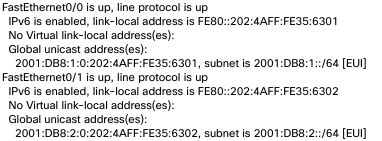
\includegraphics[width=.9\linewidth]{./router0.png}
\end{center}

Router1:
\begin{center}
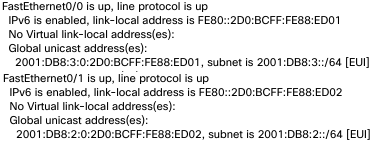
\includegraphics[width=.9\linewidth]{./router1.png}
\end{center}

\begin{enumerate}
\item Una dirección IPv6 tiene 128 bits.
\item El prefijo es 2001:DB8:1::/64 y la ID de la interface es 202:4AFF:FE35:6301
\item La MAC es 0002.4A35.6301. El ID de la interface se forma dividiendo la MAC en dos partes de 24 bits y agregando en el medio FFFE. Éste es el formato EUI-64.
\end{enumerate}

c.

Router0:
\begin{center}
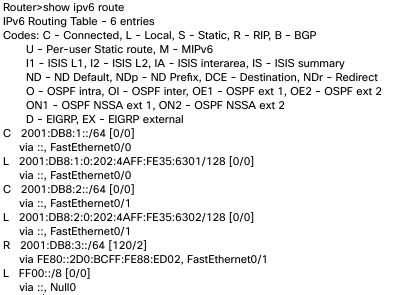
\includegraphics[width=.9\linewidth]{./r0route.png}
\end{center}

Router1:
\begin{center}
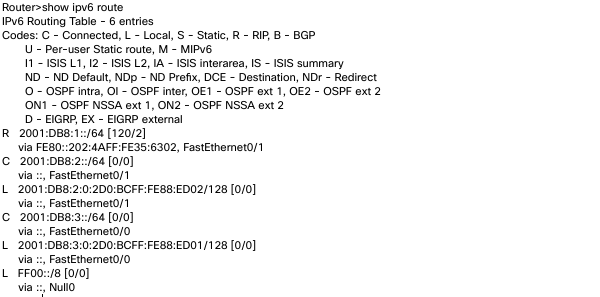
\includegraphics[width=.9\linewidth]{./r1route.png}
\end{center}

d.

\begin{center}
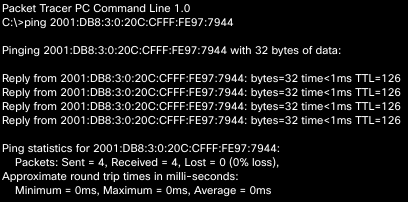
\includegraphics[width=.9\linewidth]{./ping.png}
\end{center}
\end{enumerate}
\end{document}